\section{Domande del Syllabus}

\subsection{Precisione di macchina}
Si parte da un numero reale, scritto in notazione floating point:\\
\begin{displaymath}
    x=sign(x)(0,d_1d_2....dt...)\cdot b^p
\end{displaymath}
È importante tenere a mente che la 1° cifra dopo la virgola $(d_1)$ è diversa da zero.\\
Quindi si scrive il numero arrotondato a $t$ cifre di mantissa, e si scrive la definizione formale di \underline{arrotondamento}.\\
Poi diciamo che la precisione di macchina è l'errore relativo di arrotondamento, e scriviamo l'errore di arrotondamento:
\begin{displaymath}
    \frac{|x-fl^t(x)|}{|x|},  |x| \neq 0
\end{displaymath}
Quindi stimiamo questo rapporto in due parti: prima il numeratore.\\
Le cifre dei due numeri sono uguali fino alla $t-1$, cambia dalla $t$ in poi (per l'arrotondamento), e con un esempio di può vedere che questa quantità è $\leq \frac{b^{-t}}{2}$\\
ESEMPIO: se $x=3.14$ e voglio arrotondare ai decimi, l'errore che compio è $\leq$ mezzo decimo (in questo caso di 0.04):\\
\begin{center}
    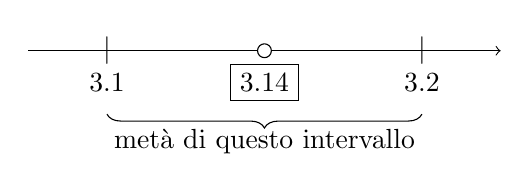
\begin{tikzpicture}
    % Retta orientata
    \draw[->] (0,0) -- (6,0);
    
    % Numeri sotto la retta
    \node at (1,-0.4) {$3.1$};
    \node[draw] at (3,-0.4) {$3.14$};
    \node at (5,-0.4) {$3.2$};
    
    % Numeri sulla retta
    \node at (1,0) {$|$};
    \node[draw, circle, fill=white, inner sep=0pt, minimum width=5pt] at (3,0) {};
    \node at (5,0) {$|$};
    
    % Parentesi graffa orizzontale
    \draw[decorate,decoration={brace,amplitude=5pt,mirror},xshift=0pt,yshift=-3pt] (1,-0.7) -- (5,-0.7) node[midway,below,yshift=-2pt] {metà di questo intervallo};
    \end{tikzpicture}
\end{center}
Ora stimiamo il denominatore. Sappiamo che è una quantità positiva (c'è il valore assoluto), è $\neq$ 0, e la prima cifra decimale $(d_1)$ deve essere diversa da zero. Questo serve ad evitare che ci siano più rappresentazioni dello stesso numero.\\
Quindi $|x|$ è almeno $(\geq)$ $0.1 \cdot b^p$ (non ci serve uno specifico p), ovvero $b^{-1}\cdot b^p => b^{p-1}$.\\
Siccome nella definizione di errore relativo $|x|$ "sta sotto", dobbiamo scrivere il reciproco: 
\begin{displaymath}\frac{1}{|x|}\leq \frac{1}{b^{p-1}}\end{displaymath}
Da notare il fatto che è cambiato il verso della disequazione.\\
Quindi uniamo i due pezzi, e otteniamo che:\\
\begin{center}
    \large\begin{displaymath}
        \frac{|x-fl^t(x)|}{|x|}\leq \frac{\frac{b^{-t}}{2}}{b^{p-1}}= \frac{b^{p-t+1-p}}{2}= \frac{b^{1-t}}{2}
    \end{displaymath}
\end{center}
Che è la nostra precisione di macchina.
\newpage

\subsection{Analisi di stabilità delle operazioni}
Questa è la più lunga di tutte le dimostrazioni, ma:
\begin{itemize}
    \item all'esame il prof ne chiede sempre metà (solitamente moltiplicazione e divisione oppure somma algebrica)
    \item Non serve impararsi tutto a memoria: gran parte del testo sono operazioni algebriche. Si utilizza la diseguaglianza triangolare e si moltiplica/divide per una certa quantità (questo nel caso della somma algebrica, nella moltiplicazione si somma/sottrae).
    \item Si inizia dalla definizione, ovvero l'errore relativo che ho su un'operazione con numeri approssimati:\begin{displaymath}\varepsilon _{x\star y}=\frac{|x\star y - \widetilde{x}\star \widetilde{y}|}{|x \star y|} \end{displaymath}  Dove al posto di $\star$ si mette una delle operazioni, e $\widetilde{x}$, $\widetilde{y}$ (con la tilde) sono i numeri approssimati.
    \item La sottrazione (ovvero la somma algebrica nel caso in cui il segno dei due numeri è diverso) è l'unica operazione instabile (quando $x$ e $y$ sono vicini in termini relativi)
\end{itemize}

\newpage
\subsection{Convergenza del metodo di bisezione}
Questa è la prima domanda in cui il prof inizia a utilizzare la lettera $\xi$ (csi), che semplicemente indica la soluzione che stiamo cercando. Invece con $x$ (oppure $x_n$) indica la "soluzione" che abbiamo trovato a una certa iterazione. In generale, più iterazioni abbiamo e più la nostra $x$ si avvicina a $\xi$.\\
Con \underbar{convergenza} di un metodo (in questo caso la bisezione) si intende il fatto che, facendo iterazioni, ci avviciniamo sempre di più alla soluzione $\xi$, lo "zero" della funzione.\\
Il metodo di bisezione funziona applicando iterativamente il \underbar{teorema degli zeri} (o teorema di Bolzano).
\begin{center}
    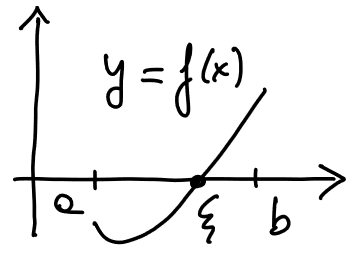
\includegraphics[scale=0.6]{./res/img/bisezione1.png}
\end{center}
Se ho una funzione continua in un intervallo $[a,b]$ e $f(a) \cdot f(b)\leq 0$ (ovvero hanno segno opposto), allora esiste un punto $\xi$, con $f(\xi)=0$, che appartiene all'intervallo $(a,b)$.\\
Il metodo consiste nell'individuare il punto medio, e continuare il procedimento sulla metà dell'intervallo in cui vale la condizione che i due estremi hanno segno opposto.\\
Esempio:
\begin{center}
    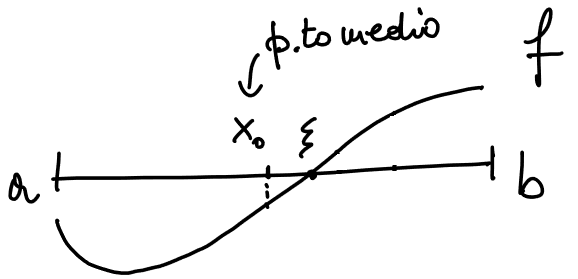
\includegraphics[scale=0.6]{./res/img/bisezione2.png}
\end{center}
In questa funzione abbiamo come estremi $a, b$. Individuiamo il \underbar{punto medio} $x_0$, e la successiva iterazione la facciamo sul semintervallo $[a,x]$, perché $f(a) f(x_0)\leq 0$.\\
Il punto medio è $x_n=\frac{a_n+b_n}{2}$.\\
Poi si individuano tre successioni: ${a_n}$, ${b_n}$, ${x_n}$, tali che:
\begin{itemize}
    \item $|\xi-a_n|\leq b_n-a_n = \frac{b-a}{2^n}$
    \item $|\xi-b_n|\leq b_n-a_n = \frac{b-a}{2^n}$
    \item $|\xi-x_n|\leq \frac{b_n-a_n}{2} = \frac{b-a}{2^{n+1}}$
\end{itemize}
$\frac{b-a}{2^n}$ è la lunghezza dell'intervallo $b_n-a_n$, mentre $\frac{b-a}{2^{n+1}}$ è la distanza tra il punto medio e $\xi$, e non può superare metà dell'intervallo $b_n-a_n$.\\
Quindi si dimostra che le tre successioni convergono ad uno zero, utilizzando il teorema dei carabinieri:\\
\begin{displaymath}
    0 \leq |\xi-a_n|, |\xi-b_n| < \frac{b-a}{2^n}\to 0, n \to \infty \overset{teor. carabinieri}{\implies} |\xi-a_n|, |\xi-b_n| \to 0, n \to \infty
\end{displaymath}
Qui semplicemente diciamo che $|\xi-a_n|, |\xi-b_n|$ sono due quantità positive (per via dei valori assoluti), e da quello che abbiamo detto prima sono $\leq$ di $ \frac{b-a}{2^n}$.\\
Calcolando il $\lim_{n\to \infty} \frac{b-a}{2^n}$ otteniamo che è zero. Quindi possiamo utilizzare il teorema dei carabinieri per dire che le due successioni tendono a zero.\\
Lo stesso ragionamento lo utilizziamo per la terza successione:
\begin{displaymath}
    0 \leq |\xi-x_n|< \frac{b-a}{2^{n+1}}\implies |\xi-x_n| \to 0, n\to \infty
\end{displaymath}

\subsection{Stima dell'errore con residuo pesato (bisezione)}
Prima di tutto è bene tenere a mente perché il residuo non pesato (detto anche stima a priori) non è una buona stima dell'errore.\\
Poi, partiamo dalle ipotesi: sono le stesse del metodo di bisezione, con l'aggiunta che la funzione, oltre a essere continua in $[a,b]$, deve anche essere derivabile, e questa derivata deve essere $\neq 0$ in tutto l'intervallo.\\
Quindi abbiamo che l'errore 
\begin{displaymath}
    e_n=\frac{f(x_n)}{f'(z_n)}
\end{displaymath}
Dove $z_n$ è un punto che appartiene all'intervallo $(x_n, \xi)$, ma non sappiamo esattamente quanto vale.\\
Si dimostra utilizzando il teorema del valor medio (detto anche teorema di Lagrange), che dice che se $f$ è continua in $[a,b]$ e derivabile in $(a,b)$, allora esiste un punto $z$ in $(a,b):$ la retta che passa per $f(a)$ e $f(b)$ è parallela alla tangente in $z$:
\begin{displaymath}
    \frac{f(b)-f(a)}{b-a}=f'(z)
\end{displaymath}

\begin{center}
    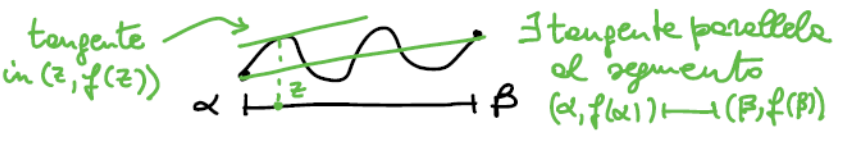
\includegraphics[scale=0.7]{./res/img/lagrange1.png}
\end{center}
Siccome $z_n$ è nell'intervallo $(x_n,\xi)$, e $x_n$ tende a $\xi$, allora la derivata di $z_n$ ha un valore molto vicino a quello della derivata di $\xi$.\\
Con la notazione $int(x_n,\xi)$ indichiamo un intervallo che ha come estremi $x_n$ e $\xi$, ma non sappiamo quale dei due è più grande.\\
La dimostrazione si fa con un'applicazione del teorema del valor medio. Supponiamo di essere nel caso in cui $\xi < xn$ (l'altro caso è analogo), e quindi $a=\xi$, $b=x_n$, e "sostituiamo" questi valori nella formula del valor medio:\\
\begin{displaymath}
    %f(x_n)-f(\xi)=f'(z_n)(x_n-\xi)
    f(x_n)-f(\xi)=f'(z_n)(x_n-\xi) \xrightarrow{}\text{il denominatore lo portiamo sopra}
\end{displaymath}
Che si può riscrivere come
\begin{displaymath}
    |x_n-\xi|=\frac{f(x_n)}{f'(z_n)}=e_n
\end{displaymath}
\subsection{Convergenza globale del metodo di Newton}
Il metodo di Newton è un altro metodo iterativo per trovare gli zeri di una funzione. Rispetto alla bisezione converge molto più rapidamente, ma ha bisogno di ipotesi più forti\footnote[1]{vedi lezione 9 - confronto tra bisezione e metodo di Newton}.\\
Questo è il metodo di Newton:
\begin{align*}
    &\systeme{y = 0, y = f(x_n)+f'(x_n)(x-x_n)}  \quad \Rightarrow \quad x_{n+1} = x_n-\frac{f(x_n)}{f'(x_n)}
\end{align*}
Queste sono le ipotesi:
\begin{equation*}
    \begin{cases}
        f \in C^2[a,b] & \text{la funzione ha derivata seconda e } f''(x) \text{ è continua} \\
        f(a)f(b) < 0   & f(a) \text{ e } f(b) \text{ hanno segno opposto}\\
        f''(x)>0 \forall x \in [a,b] & \text {dimostriamo solo il caso di concavità stretta}\\
        x_0: f(x_0)f''(x_0)>0 & \text{punto iniziale "scelto bene"}
    \end{cases}
    \end{equation*}
Riguardo la scelta del punto iniziale, è una condizione importante, altrimenti il metodo non converge alla soluzione.\\
Nella dimostrazione vengono illustrati graficamente quattro casi differenti, in base al segno di $f''(x)$ e se $f(a)>f(b)$ (oppure viceversa). Basta farne solo uno (gli altri sono uguali), per comodità scegliamo il primo, che è quello che tratta anche il prof. a lezione:\newline
CASO \circled{1}:
\begin{center}
    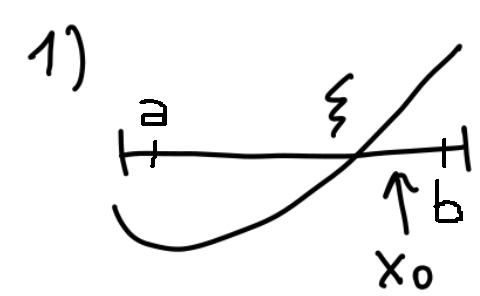
\includegraphics[scale=0.5]{./res/img/newton1.png}
\end{center}
\begin{itemize}
    \item $f(a)<0, f(b)>0$
    \item $f''(x)>0 \forall x \in [a,b]$
    \item $x_0 \in (\xi,b]$
\end{itemize}
Dobbiamo dimostrare due cose: innanzitutto, per induzione, se l'$n$-esimo termine appartiene all'intervallo $(\xi,b]$, allora lo stesso vale per il termine $n+1$-esimo. La dim. si fa a parole.\\
Poi bisogna dimostrare che ${x_n}$ è decrescente. Qui si riprende la definizione di metodo di Newton:
\begin{displaymath}
    x_{n+1} = x_n-\frac{f(x_n)}{f'(x_n)}
\end{displaymath}
Guardando il grafico del caso \circled{1} si capisce che, nell'intervallo $(\xi,b]$, $f(x)$ è sempre $>0$.\\
Stessa cosa per $f'(x_n)$, che potrebbe essere negativo solo se $f''(x)$ cambiasse segno in $(\xi,b]$, cosa che escludiamo (vedi le ipotesi iniziali).\\
Quindi $x_{n+1}$ è dato da $x_n$ a cui viene sottratta una quantità positiva. Questo è sufficiente per dire che la successione ${x_n}$ è decrescente.\\
Infine diciamo che, visto che la successione è decrescente, per il teorema della monotonia diciamo che il limite (per $n\rightarrow \infty$) della successione è il suo estremo inferiore, che il prof indica con la lettera $\eta$.\\
Quindi passiamo al limite della formula, e diciamo che:
\begin{displaymath}
    \eta=\lim_{}x_{n+1}=\lim_{}\left ( x_n-\frac{f(x_n)}{f'(x_n)} \right )
\end{displaymath}
Dopo un po' di proprietà di limiti e continuità otteniamo
\begin{displaymath}
    \eta= x_n-\frac{f(\eta))}{f'(\eta)}
\end{displaymath}
Infine diciamo che
\begin{displaymath}
    \frac{f(\eta)}{f'(\eta)}=0 \Rightarrow f(\eta)=0\Rightarrow \eta = \xi
\end{displaymath}

\subsection{Ordine di convergenza del metodo di Newton}
Le ipotesi di partenza sono le stesse della domanda precedente, con l'aggiunta che la derivata prima deve essere $\neq 0$ per ogni x contenuto in un sottointervallo di $[a,b]$. Questo ci servirà più avanti, per evitare la divisione per zero.

\subsection{Ordine di convergenza delle iterazioni di punto fisso}

\subsection{Esistenza e unicità dell'interpolazione polinomiale}

\subsection{Convergenza uniforme dell'interpolazione lineare a tratti}

\subsection{Stime di condizionamento: perturbazione termine noto} 
Partiamo innanzitutto da alcune definizioni, utili ad aggiungere un po' di contesto:\\
\underline{NORMA VETTORIALE}: La norma indica il modulo (lunghezza) del vettore, si utilizza quando bisogna confrontare la grandezza di diversi vettori o matrici.\footnote[2]{\url{https://www.youmath.it/lezioni/algebra-lineare/matrici-e-vettori/882-norma-e-prodotto-scalare.html}}\\
\underline{SISTEMA LINEARE}: è un sistema di equazioni lineari, ossia un sistema costituito da equazioni in più incognite ove ogni incognita compare con esponente 1. Nel nostro caso avremo un sistema di $n$ equazioni in $n$ incognite (questo ci serve perché la matrice dei coefficienti $A$ deve essere invertibile).\\
La \underline{perturbazione} è un errore generico (non sappiamo se è dovuto ad approssimazioni o ha altre cause), e va a modificare il risultato. Nel nostro caso, abbiamo che la perturbazione è sul termine noto, che è $b$, quindi il termine noto con l'errore lo indichiamo con $\tilde{b}$, definito nel seguente modo:\\
$\tilde{b}=b+\delta b$ ovvero b perturbato è determinato dal valore originale ($b$) a cui aggiungiamo l'errore ($\delta b$), che può essere una quantità positiva o negativa.\\
Quindi, avendo un errore sul termine noto del sistema, questo avrà conseguenze anche sulle soluzioni dello stesso, e quindi la perturbazione sarà presente anche sul vettore delle soluzioni $x$.\\
Se il sistema non affetto da errori è $Ax=b$, il sistema perturbato sarà $A\tilde{x}=\tilde{b}$\\
Il \underline{condizionamento} è la risposta del sistema agli errori sui dati:se il sistema è mal condizionato, un piccolo errore sui dati comporta ad una grande differenza sulla soluzione.\\
Nella dimostrazione\footnote[3]{Per approfondire: \url{http://dm.unife.it/~tinti/Didattica/Labcn/lucidi9.pdf}} non è obbligatorio scrivere entrambe le disuguaglianze fondamentali (visto che utilizziamo solo la prima):\\
$\lVert Ax \rVert \leq \lVert A \rVert \cdot \lVert x \rVert \quad $1° disuguaglianza fondamentale\\
Ora scriviamo le ipotesi:
\begin{itemize}
    \item $A \in {\rm I\!R}^{n\times n}$ non singolare
    \item $x \in {\rm I\!R}^n$ soluzione del sistema $Ax=b$
    \item $\tilde{x}=x+\delta x$ soluzione del sistema $A\tilde{x}=\tilde{b}$, con $\tilde{b}=b+\delta b$, $b \neq 0$
\end{itemize}
Fissata una norma $\lVert \cdot \rVert \in {\rm I\!R}$, affermiamo che vale la seguente stima dell'errore relativo su $x$ (le norme vanno messe in tutte le disuguaglianze della dimostrazione):\\
\begin{displaymath}
    \frac{\lVert \delta x \rVert}{\lVert x \rVert} \leq k(A)\frac{\lVert \delta b \rVert}{\lVert b\rVert} \quad \text{con} \quad k(A)=\lVert A \rVert \cdot \lVert A^{-1}\rVert
\end{displaymath}
La dimostrazione inizia osservando che il sistema di partenza può essere scritto come $x=A^{-1}b$, perché $A^{-1}$ è l'inversa di A, ovvero $A^{-1}=\frac{1}{A}$.
\begin{align*}
    &\systeme{\tilde{x} = x+\delta x, \tilde{x} = A^{-1}\tilde{b}=A^{-1}(b+\delta b) = A^{-1}b + A^{-1}\delta b}  \quad \Rightarrow \quad \highlightRED{\lVert \delta x \rVert} = \lVert A^{-1}\delta b \rVert \leq \raisebox{-10pt}{*} \highlightRED{\lVert A^{-1} \rVert \cdot \lVert \delta b \rVert}
\end{align*}
* 1° disusuaglianza fondamentale\\
$\lVert \delta x \rVert = \lVert A^{-1}\delta b \rVert$ la otteniamo dalle ipotesi iniziali e da un pezzo della dimostrazione. Infatti $\delta x=x+\tilde{x}$. Poco fa abbiamo visto che $\tilde{x}=A^{-1}\tilde{b}$, che è uguale a $x+A^{-1}\delta b$. A questo punto otteniamo\\ $x+\delta x=x+A^{-1}\delta b$. A questo punto semplifichiamo $x$ e mettiamo le norme.\\
Finora abbiamo stimato $\lVert \delta x \rVert$, adesso stimiamo il denominatore, $\lVert \frac{1}{x} \rVert$, da sotto $\lVert x \rVert$:\\
\begin{displaymath}
    \lVert b \rVert=\lVert Ax \rVert \leq \raisebox{-10pt}{*} \lVert A \rVert \cdot \lVert x \rVert
\end{displaymath}
* 1° disusuaglianza fondamentale\\
Da cui
\begin{displaymath}
    \lVert x \rVert \geq \frac{\lVert b \rVert}{\lVert A \rVert}
\end{displaymath}
e
\begin{displaymath}
    \highlightCYAN{\frac{1}{\lVert x \rVert} \leq \frac{\lVert A \rVert}{\lVert b \rVert}}
\end{displaymath}
Perciò (si mettono insieme le parti colorate per ritornare alla stima iniziale):
\begin{displaymath}
    \frac{\highlightRED{\lVert \delta x \rVert }}{\lVert x \rVert } \leq \frac{\highlightRED{\lVert A^{-1} \rVert \cdot \lVert \delta b \rVert }}{\highlightCYAN{\lVert x \rVert }} \leq \lVert A^{-1} \rVert  \cdot \highlightCYAN{\lVert A \rVert} \cdot \frac{\lVert \delta b \rVert }{\highlightCYAN{\lVert b \rVert }} = k(A)\cdot \frac{\lVert \delta b \rVert }{\lVert b \rVert }
\end{displaymath}